\documentclass[a4paper, 11pt]{article}

%%% Работа с русским языком
\usepackage{cmap}					% поиск в PDF
\usepackage{mathtext} 				% русские буквы в формулах
\usepackage[T2A]{fontenc}			% кодировка		% кодировка исходного текста
\usepackage[english,russian]{babel}	% локализация и переносы

%%% Дополнительная работа с математикой
\usepackage{amsfonts,amssymb,amsthm,mathtools} % AMS
\usepackage{amsmath}
\usepackage{icomma} % "Умная" запятая: $0,2$ --- число, $0, 2$ --- перечисление

\usepackage{indentfirst} % Красная строка в начале абзацев

\usepackage{setspace} % Междустрочный интервал
\singlespacing

\usepackage[left=20mm, top=10mm, right=10mm, bottom=25mm, nohead, footskip=7mm]{geometry} % поля документа

%% Номера формул
%\mathtoolsset{showonlyrefs=true} % Показывать номера только у тех формул, на которые есть \eqref{} в тексте.

%% Шрифты
\usepackage{euscript}	 % Шрифт Евклид
\usepackage{mathrsfs} % Красивый матшрифт

%% Перенос знаков в формулах (по Львовскому)
\newcommand*{\hm}[1]{#1\nobreak\discretionary{}
    {\hbox{$\mathsurround=0pt #1$}}{}}

%%% Работа с картинками
\usepackage{graphicx}  % Для вставки рисунков
\graphicspath{{images/}{images2/}}  % папки с картинками
\setlength\fboxsep{3pt} % Отступ рамки \fbox{} от рисунка
\setlength\fboxrule{1pt} % Толщина линий рамки \fbox{}
\usepackage{wrapfig} % Обтекание рисунков и таблиц текстом

%%% Работа с таблицами
\usepackage{array,tabularx,tabulary,booktabs} % Дополнительная работа с таблицами
\usepackage{longtable}  % Длинные таблицы
\usepackage{multirow} % Слияние строк в таблице


\usepackage[utf8]{inputenc}
\usepackage[russian]{babel}
\usepackage{amsmath,amsfonts,amssymb,amsthm,mathtools} %AMS

\usepackage{hyperref}  % Гиперссылки
\usepackage[usernames,dvipsnames,svgnames,table,rgb]{xcolor}
\usepackage{enumitem} %Для нумерации списков
\usepackage{multicol} % Несколько колонок
\usepackage{multirow} % Несколько строк
%\usepackage{caption} % отступы между названием и объектом
%\captionsetup[images]{skip=2ex}

\usepackage{dsfont}

\DeclareMathOperator*{\argmax}{arg\,max}

\hypersetup{
    unicode=true,
    pdftitle={cheat_sheet}, % Заголовок
    pdfauthor={Кузьмин Никита, ММП 317},
    pdfcreator={Кузьмин Никита, ММП 317},
    colorlinks=false, % false - ссылки в рамках; true - цветные ссылки
    linkcolor=red,   % внутренние ссылки
    citecolor=green, % на библиографию
    filecolor=magenta, % на файлы
    urlcolor=blue % на URL
}

\usepackage{fancyhdr}% загрузим пакет
%\pagestyle{fancy}% применим колонтитул

\begin{document}
    
%    \thispagestyle{empty}
%    \begin{center}
%        \textit{Московский Государственный Университет имени М. В. Ломоносова\\
%            Факультет выислительной математики и кибернетики}
%        \vspace{0.5ex}
%        \vspace{30ex}
%        
%        Отчет по заданию №1 "\textbf{Метрические алгоритмы классификации}". Алгоритм k ближайших соседей
%        
%    \end{center}
%    \vspace{13ex}
%    \begin{flushright}
%        \noindent % Убирает красную строку
%        \vfill
%        \textit{Кузьмин Н. В.}
%        \\
%        \textit{студент кафедры ММП \\ 317 группа}
%        
%    \end{flushright}
%    \begin{center}
%        Октябрь,
%        
%        2019
%    \end{center}
 %   \newpage
    %\begin{enumerate}
    %    \item Введение
    %    \item Эксперименты
    %    \begin{enumerate}[label*=\arabic*.]
    %        \item Скорость поиска ближайших %соседей
    %        \item Зависимость точности %модели от количества соседей и %метрики
    %        \item Сравнение точности %взвешенного метода и метода без %весов
    %        \item Анализ модели с лучшим %качеством
    %        \item Применение трансформаций %к тренировочной выборке
    %         \begin{enumerate}[label*=\arab%ic*.]
    %            \item Повороты
    %            \item Смещения
    %            \item Фильтр Гаусса
    %         \end{enumerate}
    %         \item Применение трансформаций %к тестовой выборке
    %         \begin{enumerate}[label*=\arab%ic*.]
    %            \item Повороты
    %            \item Смещения
    %            \item Фильтр Гаусса
    %         \end{enumerate}
    %    \end{enumerate}
    %    \item Бонусная часть
    %    \item Выводы
    %\end{enumerate}
    \hfill Кузьмин Никита, ММП, 317.
    
    \center \Large Отчет по заданию №1 "\textbf{Метрические алгоритмы классификации}". Алгоритм k ближайших соседей
    \tableofcontents
    
    \newpage
    \section{Введение}
    В этом документе представлен отчет о проделанных экспериментах по практическому заданию №1, анализ результатов. 
    
    Краткое описание задания: необходимо реализовать алгоритмы $k$ ближайших соседей и кросс-валидации, провести эксперименты с датасетом изображений цифр \textbf{MNIST}.
    
    
    \section{Эксперименты}
    В этом блоке приведены все обязательные эксперименты, которые изложены в формулировке задания.
    \subsection{Скорость поиска ближайших соседей}
    \subsubsection{Дизайн эксперимента:}
    Были протестированы 4 алгоритма поиска 5 ближайших соседей с разными размерами признакового пространства:
    
    Алгоритмы: \hspace{15em} Размеры признакового пространства: % добавить еще маркированный список
    \begin{itemize}
        \begin{multicols}{2}
            \item \text{<<my\_own>>}
            \item \text{<<brute>>}
            \item \text{<<kd\_tree>>}
            \item \text{<<ball\_tree>>}
            \item 10
            \item 20
            \item 100
        \end{multicols}
    \end{itemize}
%    \subsubsection{Ожидания}
%    Ожидается, что <<kd\_tree>>, <<ball\_tree>> будут очень хорошо работать для маленького количества признаков, но с увеличением размерности признакового пространства произойдет резкое увеличение скорости работы.
    \subsubsection{Результаты}
    Подробные результаты экспериментов приведены в таблице \ref{exp1:table}:
    \\
        \begin{table}[h]
            \begin{center}
                \caption{Результаты эксперимента №1} \label{exp1:table}
                \begin{tabular}{|c|c|r|} 
                    \hline 
                    размерность & алгоритм & время работы \\ 
                    \hline
                    10 & my\_own & 68.07 \\ 
                    \cline{2-3} 
                    & brute & 7.84 \\ 
                    \cline{2-3} 
                    & \textbf{kd\_tree} & \textbf{0.44} \\ 
                    \cline{2-3} 
                    & ball\_tree & 1.72 \\ 
                    \cline{2-3} 
                    \hline 
                    20 & my\_own & 76.82 \\ 
                    \cline{2-3}  
                    & brute & 7.95 \\ 
                    \cline{2-3}  
                    & \textbf{kd\_tree} & \textbf{1.40} \\ 
                    \cline{2-3} 
                    & ball\_tree & 6.63 \\ 
                    \hline 
                    100 & my\_own & 78.31 \\ 
                    \cline{2-3}  
                    & \textbf{brute} & \textbf{8.28} \\ 
                    \cline{2-3} 
                    & kd\_tree & 82.76 \\ 
                    \cline{2-3}
                    & ball\_tree & 97.67 \\
                    \hline
                \end{tabular} 
            \end{center}
        \end{table}
    %%вставить табличку
    \subsubsection{Выводы}
    Самым стабильным алгоритмом оказался <<brute>>, который практически не деградирует с ростом размерности. Как и ожидалось, алгоритмы, реализованные на деревьях, сильно замедлились на признаковом пространстве размерности 100.
    
    \subsection{Зависимость точности модели от количества соседей и метрики}
    \subsubsection{Дизайн эксперимента}
    В этом эксперименте была рассмотрена зависимость точности и времени работы модели $k$ ближайших соседей от следующих параметров на 3 валидационных фолдах:
    \begin{itemize}
        \item $k$ от 1 до 10 (только влияние на точность).
        \item Евклидова или косинусная метрика.
    \end{itemize}
    
    
    \subsubsection{Результаты}
        Зависимость средней точности от числа соседей для различных метрик приведена на графике \ref{exp2:graph}
        
        Измерения скорости для евлидовой и косинусной метрик приведены в таблице \ref{exp2:speed}.
    \begin{figure}[h]
        \caption{}\label{exp2:graph}
        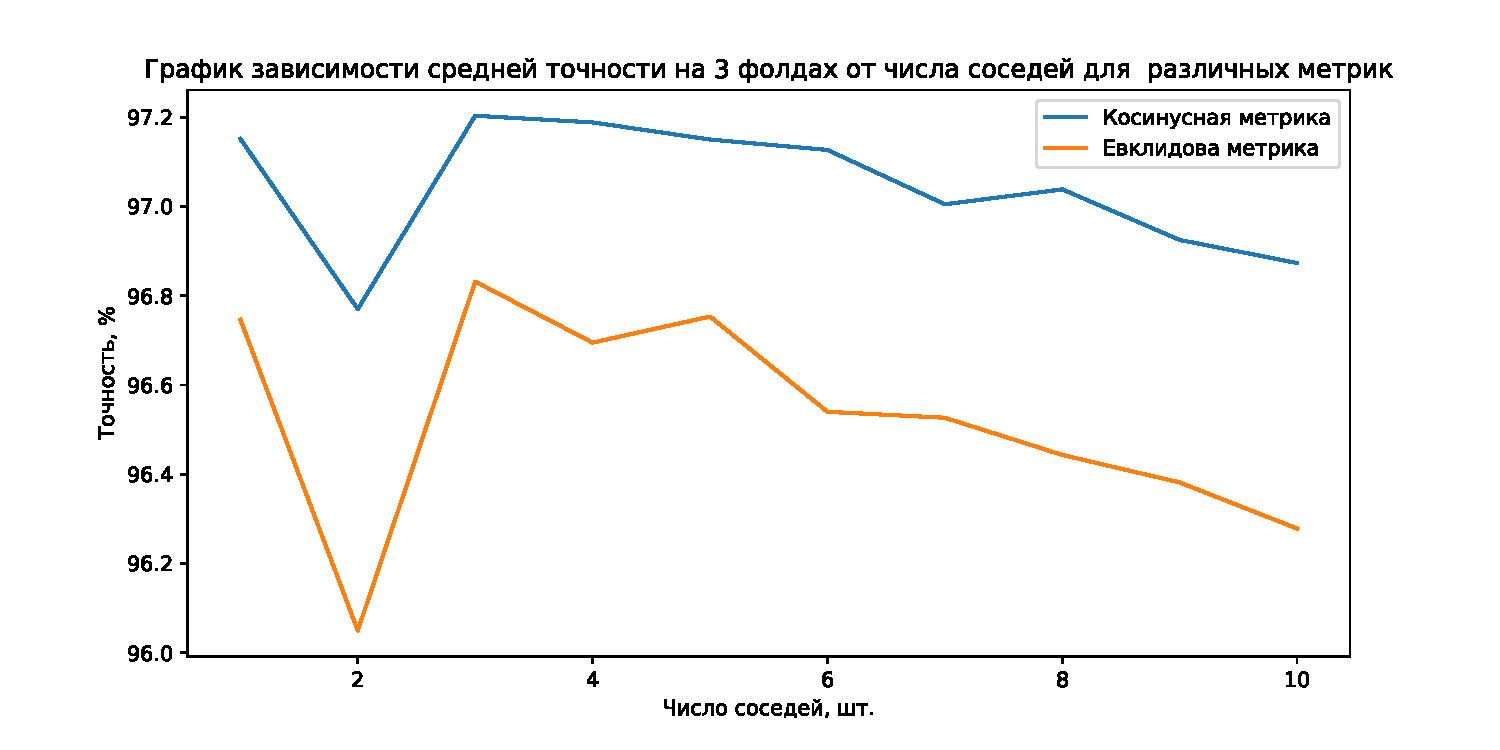
\includegraphics[width=\textwidth]{../experiment2_graph.pdf}
    \end{figure} 
    
    \begin{table}[h]
        \begin{center} 
            \caption{Скорость работы метрик (измеренная при кросс-валидации на 3 фолдах)} \label{exp2:speed}
            \begin{tabular}{|c|c|}
                \hline 
                метрика & время \\ 
                \hline 
                евклидова & 103.42 \\ 
                \hline 
                косинусная & 101.69 \\ 
                \hline 
            \end{tabular}
        \end{center}
    \end{table}
    
    \subsubsection{Выводы}
    Из графика на Рис. \ref{exp2:graph} видно, что:
        \begin{enumerate}
            \item Наибольшая точность алгоритма достигается при $k = 3$ для обеих метрик.
            \item С увеличением количества соседей (при $k \ge 5$) точность начинает убывать.
            \item Точность алгоритма с косинусной метрикой превосходит точность алгоритма с евклидовой метрикой $\forall k \in \{1, \dots, 10\}$  
        \end{enumerate} 
    
    Из таблицы \ref{exp2:speed} видно, что скорость работы алгоритмов практически не зависит от выбора данных метрик.
    \subsection{Сравнение точности взвешенного метода и метода без весов}
    \subsubsection{Дизайн эксперимента}
    Был рассмотрен метод $k$ ближайших соседей <<brute>> с косинусным расстоянием $\forall k \in \{1, \dots, 10\}$ в двух случаях:
        \begin{enumerate}
            \item Взвешенный метод
            \item Метод без весов
        \end{enumerate}
    \subsubsection{Результаты}
    Результаты эксперимента №3 приведены на графике \ref{exp3:graph}
    \begin{figure}[h]
        \caption{}\label{exp3:graph}
        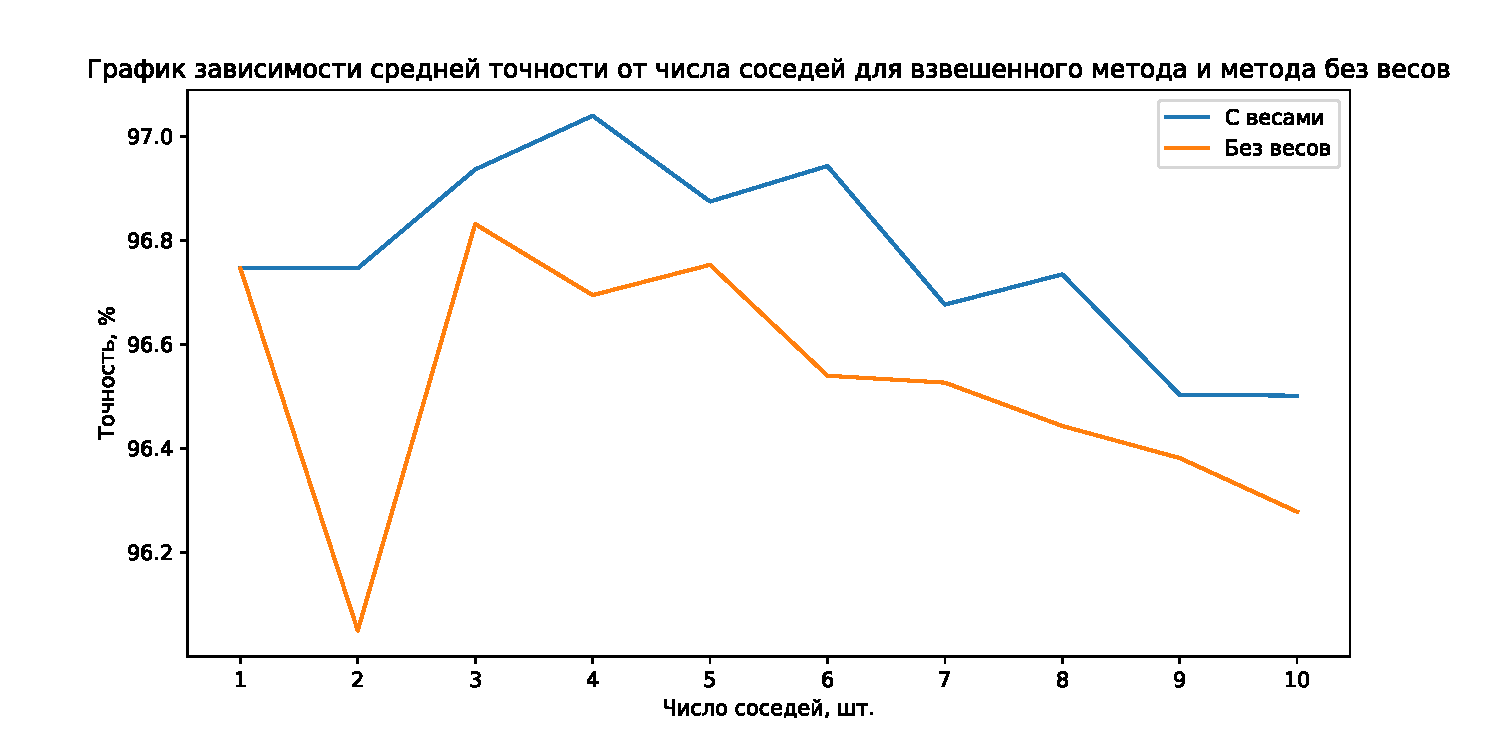
\includegraphics[width=\textwidth]{../experiment3_graph.pdf}
    \end{figure} 
    \subsubsection{Выводы}
    По графику \ref{exp3:graph} можно заметить, что взвешенный метод лучше по точности во всех случаях, кроме $k = 1$, что является логичным, так как при предсказании по одному соседу веса бесполезны.
    \subsection{Анализ модели с лучшим качеством}
    \subsubsection{Дизайн эксперимента}
    Применим лучший алгоритм (<<brute>>, косинусная метрика, с весами) к исходной обучающей и тестовой выборке и проанализируем матрицу ошибок (confusion matrix).
    \subsubsection{Результаты}
    Значения точности лучшего алгоритма на кросс-валидации, на тестовой выборке и значение точности лучшего алгоритма из интернета представлены в таблице \ref{exp4:table}. Матрица ошибок представлена на рисунке \ref{exp4:conf_matrix}, Визуализированные объекты -- на рисунке \ref{exp4:wrong_digits}\
    \begin{table}[h]
        \begin{center} 
            \caption{} \label{exp4:table}
            \begin{tabular}{|c|c|c|}
                \hline 
                алгоритм & условия & точность \\ 
                \hline 
                реализованный по заданию & кросс-валидация & 0.9741 \\ 
                \cline{2-3}
                & тестовая выборка & 0.9752 \\ 
                \hline
                сверточная нейронная сеть & тестовая выборка & 0.9979 \\ 
                \hline 
            \end{tabular} 
        \end{center}
    \end{table}
        \begin{figure}[!h]
            \begin{center}
                \begin{multicols}{2}
                    \caption{Матрица ошибок для эксперимента №4}\label{exp4:conf_matrix}
                    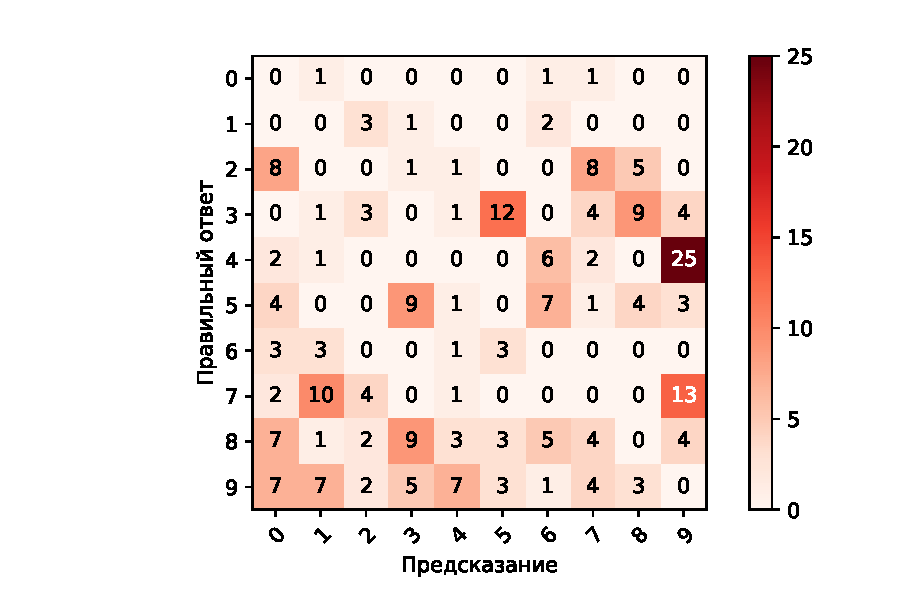
\includegraphics[width=0.5\textwidth, height=3\textheight, keepaspectratio]{../conf_matrix_experiment_4.pdf}
                    \caption{Цифры с ошибками в предсказаниях}\label{exp4:wrong_digits}
                    \vspace{5ex}
                    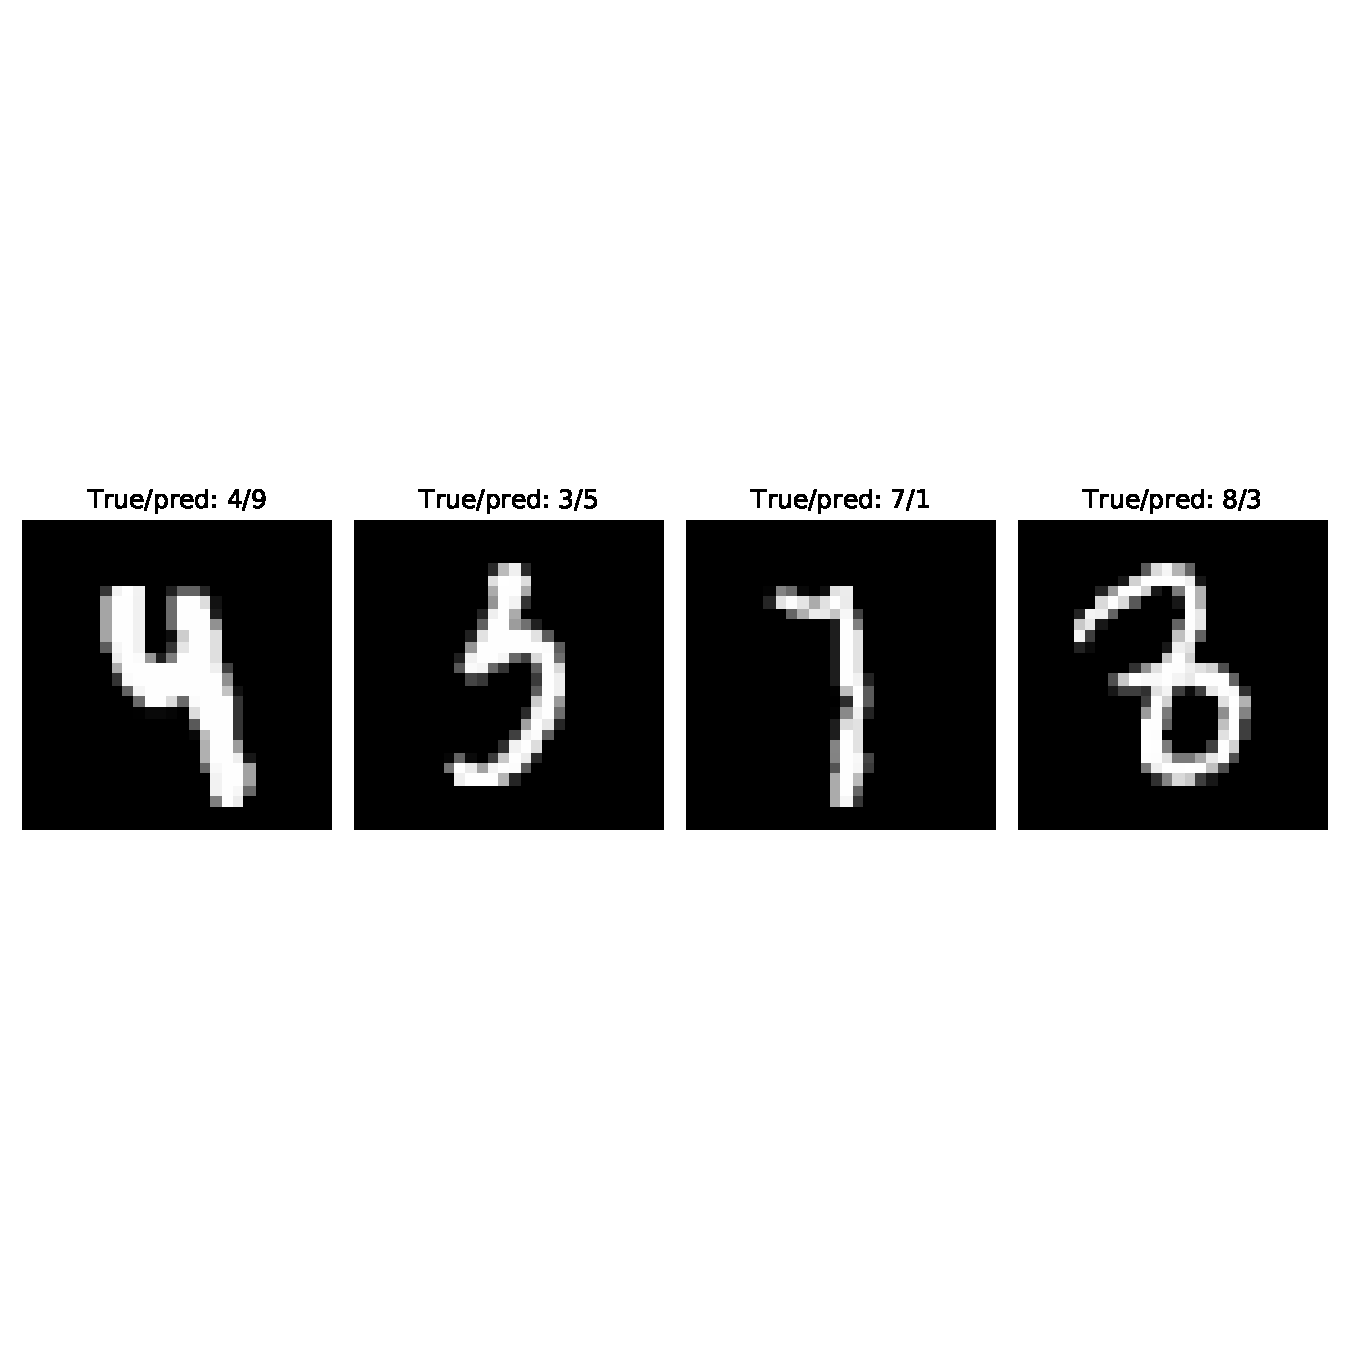
\includegraphics[width=0.5\textwidth, height=5\textheight, keepaspectratio]{../wrong_digits.pdf}
                \end{multicols}
            \end{center}
        \end{figure}
    
    \subsubsection{Выводы}
    
    Можно увидеть, что самые частые ошибки происходят на парах цифр, представленных ниже:
    \begin{itemize}
        \begin{multicols}{2}
            \item 4 и 9
            \item 3 и 5
            \item 1 и 7
            \item 3 и 8
        \end{multicols}
    \end{itemize}

    Эти пары похожи по написанию, поэтому алгоритму тяжелее отличить их друг от друга. 
    
    Рассмотрим теперь объекты, на которых произошли ошибки. У них можно заметить характерные особенности:
    \begin{enumerate}
        \item Засечки
        \item Крючки
        \item Отсутствие некоторых частей
    \end{enumerate}
    
    В представленых случаях видно, что написаннные цифры немного деформированы и похожи на другие в некоторых чертах. Эти особенности затрудняют классификацию для алгоритма.
    \\
    \subsection{Применение трансформаций к тренировочной выборке} \label{exp5}
    \subsubsection{Дизайн эксперимента}
    Пусть у нас есть $m$ элементарных преобразований: $\phi_{j}(x): \mathbb{R}^d \rightarrow \mathbb{R}^d, j \in \{1, \dots, m\}$, введем $\phi_{0}(x) = x$
    \\ 
    Создадим новую обучающую выборку:
    \[X_{new} = \left(\bigcup_{j=0}^m (\phi_{j}(x_{i}), y_{i})_{i=1}^l \right)\]
    
    Рассматриваемые преобразования\footnote{Для трансформаций тренировочной выборки использовалась библиотека \textbf{scipy}.}:
    \begin{itemize}
        \item Поворот на: $5, 10, 15^{\circ}$ (в каждую из двух сторон).
        \item Смещение на 1, 2, 3 px (по каждой из двух размерностей).
        \item Дисперсия фильтра Гаусса\footnote{Важно заметить, что функция \textbf{scipy.ndimage.gaussian\_filter} принимает в качестве аргумента $\sigma$, а не $\sigma^2$.} $\sigma^2=$ 0.5, 1, 1.5.
    \end{itemize}

    То есть применение конкретного преобразования позволяет нам расширить тренировочную выборку в 2 раза\footnote{Замечание: если размножить тренировочную выборку до вызова функции кросс-валидации, то точность сильно возрастет (особенно при взвешенном методе). Это возникает из-за того, что преобразованные объекты остаются очень близкими к исходным. Чтобы избежать этого -- нужно размножать каждый тренировочный фолд отдельно, а тестовый не трогать.}.
    \subsubsection{Результаты}
    Результаты\footnote{Кросс-валидация проводилась на первых 10000 объектах из тренировочной выборки с целью экономии времени.} приведены в таблице\ \ref{exp5:table} (только по 3 лучших параметра для каждого преобразования) и на рисунках \ref{exp5:without}, \ref{exp5:rotate},
    \ref{exp5:shift}, \ref{exp5:blur} представлены матрицы ошибок.
    \begin{table}[h]
        \caption{Точность в зависимости от преобразования} \label{exp5:table}
        \begin{center}
            \begin{tabular}{|c|c|c|}
                \hline 
                тип преобразования & параметр & точность \\ 
                \hline
                отсутствует  & $-$ & 0.945 \\
                \hline
                поворот & 5 & 0.954 \\ 
                \cline{2-3}
                & \textbf{10} & \textbf{0.956} \\ 
                \cline{2-3}
                & 15 & 0.954 \\ 
                \hline 
                сдвиг & $(1, -1)$ & 0.952 \\ 
                \cline{2-3}
                & $\textbf{(1, 0)}$ & \textbf{0.953} \\ 
                \cline{2-3}
                & $(0, 1)$ & 0.952 \\ 
                \hline 
                размытие & 0.5 & 0.957 \\ 
                \cline{2-3}
                & \textbf{1.0} & \textbf{0.960} \\ 
                \cline{2-3}
                & 1.5 & 0.959 \\ 
                \hline 
            \end{tabular}
        \end{center}
    \end{table}
    \begin{figure}[!h]
        \begin{multicols}{4} 
            \caption{Без преобр.} \label{exp5:without}
            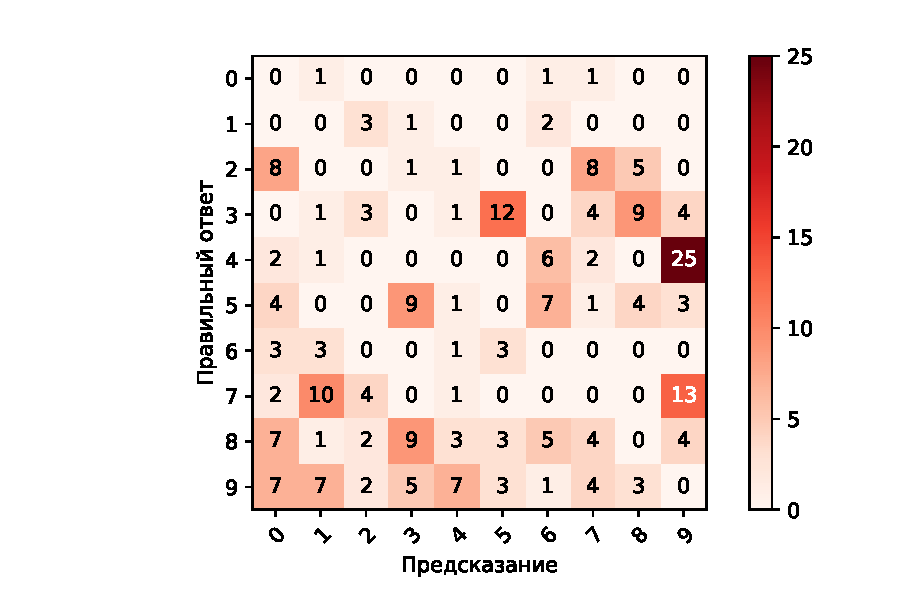
\includegraphics[width=0.25\textwidth]{../conf_matrix_experiment_4.pdf}
            \caption{Поворот на $10^{\circ}$} \label{exp5:rotate}
            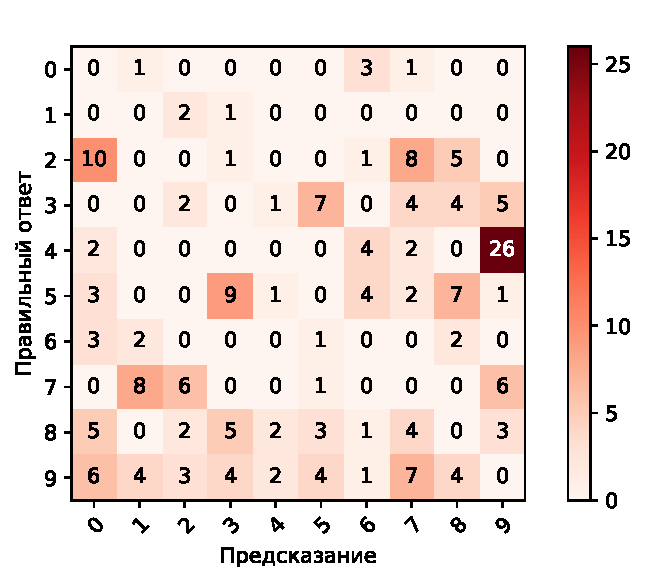
\includegraphics[width=0.25\textwidth]{../conf_matrix_experiment_5_with_rotate_10.pdf}
            \caption{Сдвиг на (1, 0) px} \label{exp5:shift}
            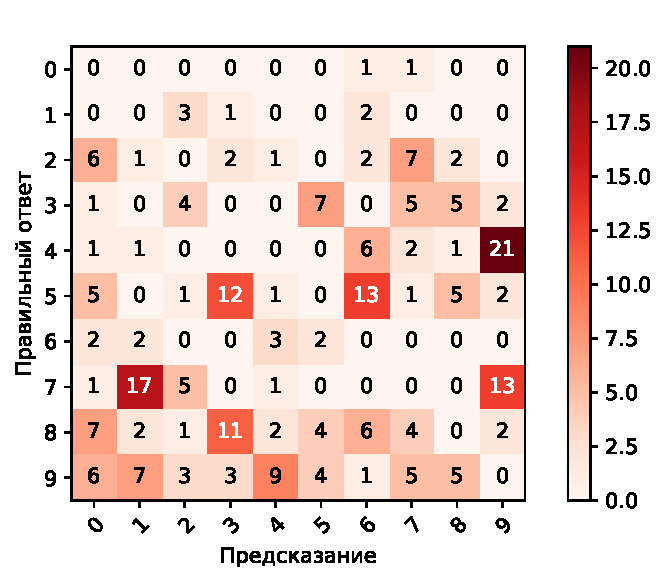
\includegraphics[width=0.25\textwidth]{../conf_matrix_experiment_with_shift_0_1.pdf}
            \caption{$\sigma^2 = 1$} \label{exp5:blur}
            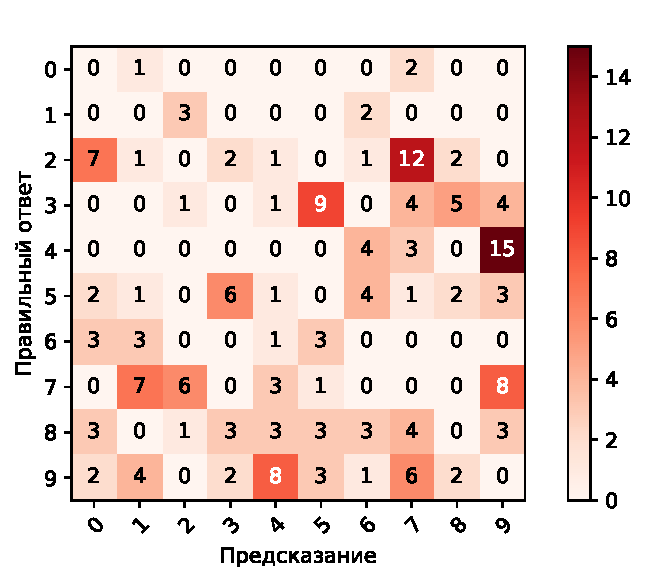
\includegraphics[width=0.25\textwidth]{../conf_matrix_experiment_with_blur_1.pdf}
        \end{multicols}
   \end{figure}
   \subsubsection{Выводы}
   Можно отметить ряд фактов, которые видны из матриц ошибок:
        \begin{enumerate}
            \item Поворот позволяет алгоритму меньше путать цифры:
            \begin{itemize}
                \item 3 с 5
                \item 7 с 9
                \item 3 с 8
            \end{itemize}
            \item Сдвиг позволяет алгоритму меньше путать цифры:
            \begin{itemize}
                \item 4 с 9
                \item 3 с 8
            \end{itemize}
            \item Размытие Гаусса позволяет алгоритму меньше путать цифры:
            \begin{itemize}
                \item 4 с 9
                \item 7 с 9
            \end{itemize}
        \end{enumerate}
   \subsection{Применение трансформаций к тестовой выборке} \label{exp6}
   \subsubsection{Дизайн эксперимента}
   Этот способ основан на преобразовании объектов тестовой выборки. Для каждого объекта тестовой выборки $x'$ получим множество объектов $\Phi(x') = \{\phi_{j}(x')|j \in\{1, \dots, m\}\}$. Введем <<расстояние>> от множества $\Phi(x')$  до объекта обучающей выборки $x$:
   \[\rho(x, \Phi(x')) = \min_{j}\{\rho(x,\phi_{j}(x')|j \in\{1, \dots, m\}\}\]
   
   Вычисление $k$ ближайших соседей для $\Phi(x')$ можно организовать следующим образом:
   \begin{enumerate}
       \item Для каждого объекта из $\Phi(x')$ найдем него $k$ ближайших соседей из обучающей выборки $X$
       \item Среди всех найденных соседей выберем $k$ объектов с наименьшим расстоянием
   \end{enumerate}
    
    По полученному множеству значений ближайших соседей вычисляется ответ алгоритма.
    \subsubsection{Результаты}
     Результаты приведены в таблице \ref{exp6:table} (только по 3 лучших параметра для каждого преобразования) и на рисунках \ref{exp6:without}, \ref{exp6:rotate},
    \ref{exp6:shift}, \ref{exp6:blur} приведены матрицы ошибок.
    \begin{table}[h]
        \caption{Точность в зависимости от преобразования} \label{exp6:table}
        \begin{center}
            \begin{tabular}{|c|c|c|}
                \hline 
                тип преобразования & параметр & точность \\ 
                \hline
                отсутствует & $-$ & 0.972 \\ 
                \hline
                поворот & -15 & 0.976 \\ 
                \cline{2-3}
                & \textbf{-10} & \textbf{0.977} \\ 
                \cline{2-3}
                & -5 & 0.974 \\ 
                \hline 
                сдвиг & $(1, -1)$ & 0.977 \\ 
                \cline{2-3}
                & $\textbf{(1, 0)}$ & \textbf{0.978} \\ 
                \cline{2-3}
                & $(3, -1)$ & 0.976 \\ 
                \hline 
                размытие & \textbf{0.5} & \textbf{0.972} \\ 
                \cline{2-3}
                & 1.0 & 0.963 \\ 
                \cline{2-3}
                & 1.5 & 0.951 \\ 
                \hline 
            \end{tabular}
        \end{center}
    \end{table}
    \begin{figure}[h]
        \begin{multicols}{4} 
            \caption{Без преобразований} \label{exp6:without}
            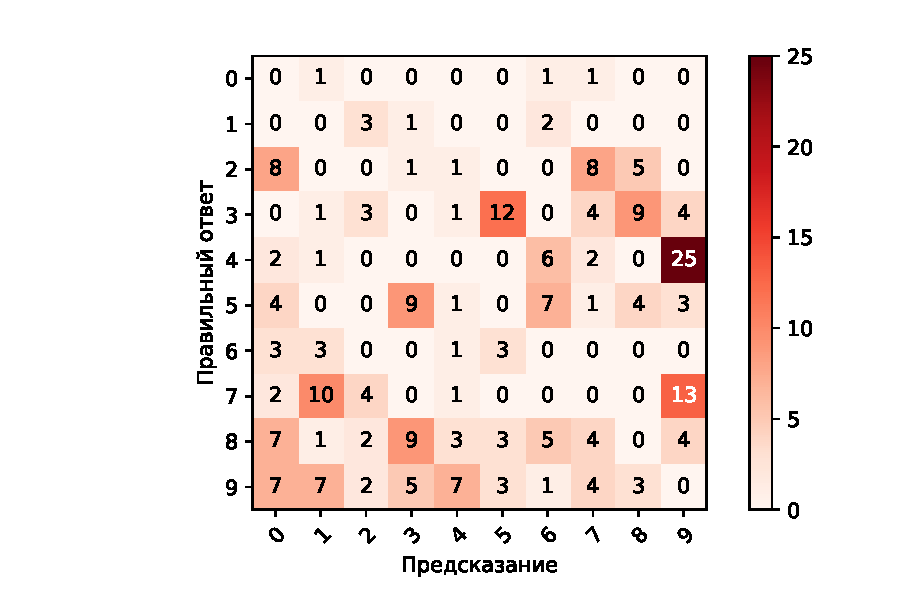
\includegraphics[width=0.25\textwidth]{../conf_matrix_experiment_4.pdf}
            \caption{Поворот на $-10^{\circ}$} \label{exp6:rotate}
            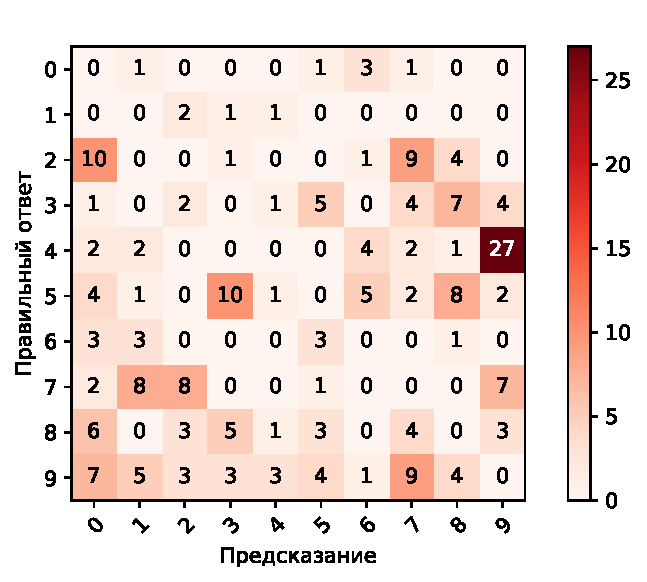
\includegraphics[width=0.25\textwidth]{../conf_matrix_experiment_6_with_rotate_-10.pdf}
            \caption{Сдвиг на (1, 0) px} \label{exp6:shift}
            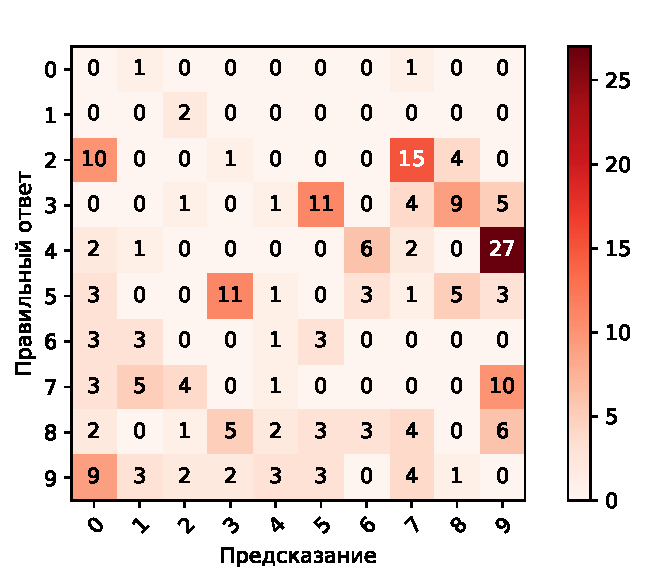
\includegraphics[width=0.25\textwidth]{../conf_matrix_experiment_6_with_shift_1_0.pdf}
            \caption{Размытие Гаусса с $\sigma^2 = 0.5$} \label{exp6:blur}
            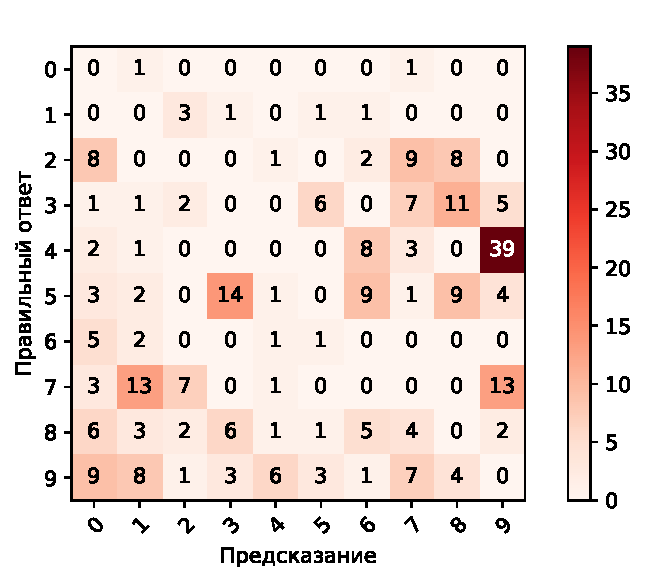
\includegraphics[width=0.25\textwidth]{../conf_matrix_experiment_6_with_blur_05.pdf}
        \end{multicols}
    \end{figure}
    \subsubsection{Выводы}
    Поворот на $10^\circ$ против часовой стрелки позволяет избавиться от значительной части ошибок, при которых модель путает 3 с 5.
    
    Сдвиг на (1, 0) px убирает ошибки, связанные с идентификацией 8 и 0, 9 и 7.
    
    Размытие Гаусса с  $\sigma^2 = 0.5$ хорошо справляется с ошибками вида 3-5, но очень плохо себя показало с 4-9. Этому есть объяснение -- 4 и 9 и без преобразований очень похожи, а после размытия Гаусса эти цифры становятся практически не различимы
    
    \section{Сравнение экспериментов 5 и 6}
    Данные эксперименты можно сравнить по двум характеристикам: 
        \begin{itemize}
            \item Затрачиваемая память:
            \\
            В условиях задачи тестовая выборка в несколько раз меньше, чем тренировочная, поэтому эффективнее увеличивать размеры именно теста.
            \item Точность алгоритма:
            \\
            Результаты измерений точности приведены в таблице \ref{comp:table}
            \begin{table}[h]
                \begin{center}
                    \caption{} \label{comp:table}
                    \begin{tabular}{|c|c|}
                        \hline 
                        номер эксперимента & точность \\ 
                        \hline 
                        \textbf{5} & \textbf{0.984} \\ 
                        \hline 
                        6 & 0.976 \\ 
                        \hline 
                    \end{tabular}
               \end{center} 
            \end{table}
            
        \end{itemize}
    \section{Дополнение}
        \subsection{Adversarial validation}
        Рассмотрим альтернативный способ валидации. Основная идея заключается в следующем: нужно добиться того, чтобы алгоритм не смог отличать тренировочную выборку от тестовой.
        
        Для реализации этого нужно сформировать новую выборку $X = X_{train} \bigcup X_{test}$, где $X_{train}, X_{test}$ -- объекты тренировочной и тестовой выборок соответственно (без меток классов). Поставим каждому объекту из $X_{train}$ в соответствие метку <<0>>, а каждому из $X_{test}$ -- <<1>>. Таким образом получена новая тренировочная выборка, к которой можно применить метод кросс-валидации для оценки модели.
        
        Выбор лучших параметров происходит на основе предсказаний модели для каждого фолда. За метрику качества удобнее всего брать площадь под кривой ошибок (\textbf{AUC ROC}). 
        
        Пусть даны две модели: $M_{1}$ и $M_{2}$; $auc\_roc_{1}$, и $auc\_roc_{2}$ -- значения площадей под кривой ошибок, усредненные по фолдам для каждой из моделей соответственно. Тогда модель $M_{1}$ считается лучше модели $M_{2}$, если выполнено следующее неравенство:
        \[|auc\_roc_{1} - 0.5| < |auc\_roc_{2} - 0.5|\]
        
        С помощью представленного способа валидации будет более результативный отбор параметров аугментаций из экспериментов \ref{exp5} и \ref{exp6}, так как он (способ) позволяет минимизировать отличия между тренировочной и тестовой выборок. 
        
        Но есть и минус у \textbf{Adversarial validation} -- обобщающая способность модели, настроенной по этому методу будет ниже, чем у модели, настроенной с помощью стандартного метода кросс-валидации, так как в первом случае она (первая модель) учитывает структуру тестовой выборки. Если новая тестовая выборка имеет совсем другое распределение, то первая модель с б\'{о}льшей вероятностью выдаст качество хуже, чем вторая.
        \subsection{Новые метрики расстояния}
                Были проведены эксперименты на лучшей модели 4-х ближайших соседей с весами на различных метриках\footnote{Все метрики, описанные ниже, реализованы в модуле \textbf{distances.py}}:
                \begin{itemize}
                    \item \textbf{Расстояние Чебышева:} $\rho(x, y) = \max_{i \in \{1, \dots, d\}}|x_{i} - y_{i}|$, где $x, y \in \mathbb{R}^d$.
                    \item \textbf{Манхэттенское расстояние:} $\rho(x, y) = \sum_{i = 1}^{d}|x_{i} - y_{i}|$, где $x, y \in \mathbb{R}^d$.
                    \item \textbf{Расстояние Минковского:} $\rho(x, y) = \left(\sum_{i = 1}^{d}|x_{i} - y_{i}|^p \right)^\frac{1}{p}$, где $x, y \in \mathbb{R}^d, p \in \mathbb{R}$.
                    
                Результаты экспериментов приведены в таблице \ref{extraexp:table} (результаты для евклидовой и косинусной метрик приведены для сравнения):
                \begin{table}[h]
                    \begin{center}
                        \caption{} \label{extraexp:table}
                        \begin{tabular}{|c|c|}
                            \hline 
                            метрика & точность \\ 
                            \hline 
                            Еквлидова & \textbf{0.9752} \\ 
                            \hline 
                            Косинусная & 0.9714 \\ 
                            \hline 
                            Чебышева & 0.8265 \\ 
                            \hline 
                            Манхэттенское расстояние & 0.9659 \\ 
                            \hline 
                            Расстояние Минсковского, p=3 & 0.9540 \\ 
                            \hline 
                        \end{tabular} 
                    \end{center}
                \end{table}
                
                \end{itemize}
       \subsection{Новые метрики качества}
            Были реализованы следующие метрики качества\footnote{Все метрики качества, описанные ниже, реализованы в модуле \textbf{metrics.py}.} алгоритма:
            \begin{itemize}
                \item \textbf{Precision:} $\frac{TP}{TP + FP}$
                \item \textbf{Recall:} $\frac{TP}{TP + FN}$
                \item \textbf{Specifity:} $\frac{TN}{TN + FP}$
                \item \textbf{F1 Score:} $\frac{2 \times Recall \times Precision}{Recall + Precision}$
            \end{itemize}
        
            Пояснение обозначений: допустим, что решается задача многоклассовой классификации, где $Y = \{y_{1}, \dots, y_{m}\}$ -- множество уникальных классов. Каждая из представленных выше метрик считается отдельно  $\forall y_{j}, j \in 1, \dots, m$. Рассмотрим их вычесление для конкретного класса $y_{j}$:
                \begin{itemize}
                    \item \textbf{TP(True Positive)} -- количество объектов класса $y_{j}$, которым алгоритм поставил метку $y_{j}$
                    \item \textbf{FP(False Positive)} -- количество объектов, \textbf{не} принадлежащих классу $y_{j}$, которым алгоритм поставил метку $y_{j}$
                    \item \textbf{FN(False Negative)} -- количество объектов класса $y_{j}$, которым алгоритм поставил метку, отличную от $y_{j}$
                    \item \textbf{TN(True Negative)} -- количество объектов, \textbf{не} принадлежащих классу $y_{j}$, которым алгоритм поставил метку, отличную от $y_{j}$
                \end{itemize}
     \subsection{Ансамбль алгоритмов}
        В данной части реализован простейший ансамбль алгоритмов\footnote{Реализован в модуле \textbf{ensemble.py}} -- пусть имеется множество моделей $M_{1}, \dots, M_{t}$ и соответсвенно их предсказания $pred_{1}, \dots, pred_{t}$  на тестовом объекте $x \in X_{test}$, где $X_{test} \in \mathbb{R}^{q\times d}$. Тогда предсказание ансабля моделей для объекта $x$ определяется следующим образом:
        \[pred(x) =\argmax_{c}{g_{c}(x)} \], где $g_{c}(x) = \sum_{m=1}^{t}w_{k} \times \mathds{1}[pred_{m}=c], c=1, 2, \dots, C$, где $w_{k}$ - некоторые веса (например, прямо пропорциональные качеству на кросс-валидации), $C$ - количество классов.
        
        В результате перебора различных вариаций ансамбля моделей удалось улучшить точность (accuracy):
        \begin{table}[h]
            \begin{center}
                \begin{tabular}{|c|c|}
                    \hline 
                    количество моделей & точность \\ 
                    \hline 
                    1 & 0.9843 \\ 
                    \hline 
                    4 & \textbf{0.9844} \\ 
                    \hline 
                \end{tabular} 
            \end{center}
       \end{table}
       
       \textbf{Анализ результата:}
       
       Ансамбль моделей помог улучшить точность, но эта разница совсем маленькая, а для её получения потребовалось в 4 раза больше времени. В рамках данной задачи лучше использовать одну модель.
\end{document}

